\documentclass[aspectratio=169]{beamer}
\usepackage[T1]{fontenc}
\usepackage[utf8]{inputenc}
\usepackage{tikz}
\usepackage{tabularx}
\usepackage[font=scriptsize]{caption}
\captionsetup[figure]{labelformat=empty}

\usetikzlibrary{tikzmark,shapes,arrows,backgrounds,fit,positioning}
\newcolumntype{C}{>{\centering\arraybackslash}X}

\addtobeamertemplate{navigation symbols}{}{
	\insertframenumber{}
	}

\title{UUB Charge and Peak histograms}
\author{
  Mauricio Su\'arez Dur\'an and Ioana~C.~Mari\c{s}
}
\institute{IIHE-ULB}

\titlegraphic{
  \begin{figure}[h]
    \centering
   
\includegraphics[width=5cm]{ulbLogo2.png}
    \hspace*{2.cm}
    
\includegraphics[width=5.5cm]{iihe.jpeg}
  \end{figure}
}

\begin{document}
\begin{frame}
  \titlepage
\end{frame}


\begin{frame}
	\frametitle{UUB Charge and Peak histograms}
  \begin{itemize}
		\item Station studied: 863
    \item Data from CDAS.
		\item {\underline {Software CDAS, pre-production version.}}
	\end{itemize}
\end{frame}

% ================
% *** For Peak ***

\begin{frame}
	\frametitle{PMT 1: UUB Peak Histogram}
	Raw UUB Peak Histogram
	\begin{figure}
		\begin{tabularx}{\textwidth}{C}
			\includegraphics[width=.7\textwidth]{../plots/uubRawPeakPMT1St863.pdf}
		\end{tabularx}
	\end{figure}
\end{frame}


\begin{frame}
	\frametitle{From UUB raw Peak histogram to the correct format}
	{\bf Applying HPeak method from IoSdStation class}
	\begin{figure}
		\centering
		\begin{tabularx}{\textwidth}{CC}
			\multicolumn{2}{l}{Each bin (j) of raw histogram is set as:} 
			\\ [2ex]
			\multicolumn{2}{l}{xp[j] = j*mult + offset;
			xp[100 + j] = 100 * mult + bigbins * j * mult + offset;} 
			\\ [2ex]
			\multicolumn{2}{l}{Here, {\it mult} and {\it bigbins} are constants and equal to 4; 
			the {\it offset} is set for each event.}
			\\
			\begin{tabular}{l}
				For event 61219267 the offset = 273, \\ 
				with a value of 273 for the first bin of \\ 
				the Peak histogram.
			\end{tabular} 
			& 
			\begin{tabular}{l}
				\includegraphics[width=.55\textwidth]{../plots/uubPeakPMT1St863.pdf}
			\end{tabular}
		\end{tabularx}
	\end{figure}
\end{frame}


\begin{frame}
	\frametitle{UUB Peak histogram Correcting for baseline}
	
	\begin{figure}
		\centering
		\begin{tabularx}{\textwidth}{CC}
			\begin{tabular}{l}
				Baseline histogram getting from \\ 
				IoSdStation::HBase
			\end{tabular}
			&
			\begin{tabular}{l} 
				\includegraphics[width=.35\textwidth]{../plots/uubBasePMT1St863.pdf}
			\end{tabular}
			\\
			\includegraphics[width=.45\textwidth]{../plots/uubPeakPMT1St863.pdf}
			&
			\includegraphics[width=.45\textwidth]{../plots/uubPeakCoorBlPMT1St863.pdf}
			\\
			Not corrected & Corrected \\
		\end{tabularx}
	\end{figure}
\end{frame}


\begin{frame}
	\frametitle{UUB Peak histogram Correcting for Offset}
	
	\begin{figure}
		\centering
		\begin{tabularx}{\textwidth}{CC}
			\includegraphics[width=.38\textwidth]{../plots/uubPeakPMT1St863.pdf}
			&
			\includegraphics[width=.38\textwidth]{../plots/uubPeakCoorOffPMT1St863.pdf}
			\\
			Not corrected & Corrected
			\\
			\begin{tabular}{l}
				Zooming to check the threshold
			\end{tabular}
			&
			\begin{tabular}{l}
				\includegraphics[width=.38\textwidth]{../plots/uubPeakCoorOffZoomPMT1St863.pdf}
			\end{tabular}
		\end{tabularx}
	\end{figure}
\end{frame}

% =======================
% *** Offset for Peak ***

\begin{frame}
	\frametitle{Offset values for UUB Peak histograms}
	{\bf For LPMT1}
	\begin{figure}
		\centering
		\begin{tabularx}{\textwidth}{CC}
			\includegraphics[width=.5\textwidth]{../plots/uubOffsetPkPMT1St863.pdf}
			&
			\includegraphics[width=.5\textwidth]{../plots/uubOffsetDiffPkPMT1St863.pdf}
		\end{tabularx}
	\end{figure}
\end{frame}
			
			
\begin{frame}
	\frametitle{Offset values for UUB Peak histograms}
	{\bf For LPMT2 and LPMT3}
	\begin{figure}
		\centering
		\begin{tabularx}{\textwidth}{CC}
			\includegraphics[width=.4\textwidth]{../plots/uubOffsetPkPMT2St863.pdf}
			&
			\includegraphics[width=.4\textwidth]{../plots/uubOffsetDiffPkPMT2St863.pdf}
			\\
			\includegraphics[width=.4\textwidth]{../plots/uubOffsetPkPMT3St863.pdf}
			&
			\includegraphics[width=.4\textwidth]{../plots/uubOffsetDiffPkPMT3St863.pdf}
		\end{tabularx}
	\end{figure}
\end{frame}



% ==================
% *** For Charge ***

\begin{frame}
	\frametitle{Applying the previous steps to UUB Charge histograms}
	{\bf Raw UUB Charge histogram}
	\begin{figure}
		\begin{tabularx}{\textwidth}{C}
			\includegraphics[width=.7\textwidth]{../plots/uubRawChargePMT1St863.pdf}
		\end{tabularx}
	\end{figure}
\end{frame}


\begin{frame}
	\frametitle{From UUB raw Charge histogram to the correct format}
	{\bf IoSdStation::HCharge}
	\begin{figure}
		\centering
		\begin{tabularx}{\textwidth}{CC}
			\multicolumn{2}{l}{Each bin (j) of the raw histogram is set as:} 
			\\ [2ex]
			\multicolumn{2}{l}{xc[j] = mult*j + offset; xc[400+j] = 400*mult + bigbins*mult*j + offset} 
			\\ [2ex]
			\multicolumn{2}{l}{Here, {\it mult}=8 and {\it bigbins}=4, both of them constants;} 
			\\
			\multicolumn{2}{l}{the {\it offset} is set for each event.} 
			\\
			\begin{tabular}{l}
				For event 61219267 offset = 0, with \\
				a value of 0 for the first bin of the \\ \\
				UUB Charge histogram.
				\\
				Not correction for baseline?
			\end{tabular} 
			& 
			\begin{tabular}{l}
				\includegraphics[width=.45\textwidth]{../plots/uubChargePMT1St863.pdf}
			\end{tabular}
		\end{tabularx}
	\end{figure}
\end{frame}


% =========================
% *** Offset for Charge ***

\begin{frame}
	\frametitle{Offset values for UUB Charge histograms}
	{\bf For LPMT1}
	\begin{figure}
		\centering
		\begin{tabularx}{\textwidth}{CC}
			\includegraphics[width=.5\textwidth]{../plots/uubOffsetChPMT1St863.pdf}
			&
			\includegraphics[width=.5\textwidth]{../plots/uubOffsetDiffChPMT1St863.pdf}
		\end{tabularx}
	\end{figure}
\end{frame}
			
			
\begin{frame}
	\frametitle{Offset values for UUB Charge histograms}
	{\bf For LPMT2 and LPMT3}
	\begin{figure}
		\centering
		\begin{tabularx}{\textwidth}{CC}
			\includegraphics[width=.4\textwidth]{../plots/uubOffsetChPMT2St863.pdf}
			&
			\includegraphics[width=.4\textwidth]{../plots/uubOffsetDiffChPMT2St863.pdf}
			\\
			\includegraphics[width=.4\textwidth]{../plots/uubOffsetChPMT3St863.pdf}
			&
			\includegraphics[width=.4\textwidth]{../plots/uubOffsetDiffChPMT3St863.pdf}
		\end{tabularx}
	\end{figure}
\end{frame}


% =====================
% *** UB Comparison ***

% *** For Peak ***

\begin{frame}
	\frametitle{Comparison with UB version, same station}
	{\bf Raw UB Peak Histogram}
	\begin{figure}
		\begin{tabularx}{\textwidth}{C}
			\includegraphics[width=.7\textwidth]{../plots/ubRawPeakPMT1St863.pdf}
		\end{tabularx}
	\end{figure}
\end{frame}


\begin{frame}
	\frametitle{From UB raw Peak histograma to the correct format}
	{\bf IoSdStation::HPeak}
	\begin{figure}
		\centering
		\begin{tabularx}{\textwidth}{CC}
			\multicolumn{2}{l}{Each bin (j) of raw Peak histogram is set as:} 
			\\ [2ex]
			\multicolumn{2}{l}{xp[j] = j*mult + offset; 
			xp[100 + j] = 100 * mult + bigbins * j * mult + offset;} 
			\\ [2ex]
			\multicolumn{2}{l}{Here, {\it mult}, {\it bigbins}, and {\it offset} are
			constants and fixed in the code with values of:}
			\\
			\multicolumn{2}{l}{mult=1, bigbins=3 y offset = 0.}
			\\ [2ex]
			\begin{tabular}{l}
				For event 61219267 offset = 57, with \\
				a value of 57 for the first of the histogram.
			\end{tabular} 
			&
			\begin{tabular}{l}
				\includegraphics[width=.48\textwidth]{../plots/ubPeakPMT1St863.pdf}
			\end{tabular}
		\end{tabularx}
	\end{figure}
\end{frame}


\begin{frame}
	\frametitle{UB Peak histogram Correcting for baseline}
	
	\begin{figure}
		\centering
		\begin{tabularx}{\textwidth}{CC}
			\begin{tabular}{l}
				Baseline from IoSdStation::HBase
			\end{tabular}
			&
			\begin{tabular}{l} 
				\includegraphics[width=.35\textwidth]{../plots/ubBasePMT1St863.pdf}
			\end{tabular}
			\\
			\includegraphics[width=.45\textwidth]{../plots/ubPeakPMT1St863.pdf}
			&
			\includegraphics[width=.45\textwidth]{../plots/ubPeakCoorBlPMT1St863.pdf}
			\\
			Not corrected & Corrected \\
		\end{tabularx}
	\end{figure}
\end{frame}


\begin{frame}
	\frametitle{UB Peak histogram Correcting for Offset}
	
	\begin{figure}
		\centering
		\begin{tabularx}{\textwidth}{CC}
			\includegraphics[width=.38\textwidth]{../plots/ubPeakPMT1St863.pdf}
			&
			\includegraphics[width=.38\textwidth]{../plots/ubPeakCoorOffPMT1St863.pdf}
			\\
			Not corrected & Corrected
			\\
			\begin{tabular}{l}
				Zooming to check the threshold
			\end{tabular}
			&
			\begin{tabular}{l}
				\includegraphics[width=.38\textwidth]{../plots/ubPeakCoorOffZoomPMT1St863.pdf}
			\end{tabular}
		\end{tabularx}
	\end{figure}
\end{frame}


% =======================
% *** Offset for Peak ***

\begin{frame}
	\frametitle{Offset values for UB Peak histograms}
	{\bf For LPMT1}
	\begin{figure}
		\centering
		\begin{tabularx}{\textwidth}{CC}
			\includegraphics[width=.5\textwidth]{../plots/ubOffsetPkPMT1St863.pdf}
			&
			\includegraphics[width=.5\textwidth]{../plots/ubOffsetDiffPkPMT1St863.pdf}
		\end{tabularx}
	\end{figure}
\end{frame}
			
			
\begin{frame}
	\frametitle{Offset values for UB Peak histograms}
	{\bf For LPMT2 and LPMT3}
	\begin{figure}
		\centering
		\begin{tabularx}{\textwidth}{CC}
			\includegraphics[width=.4\textwidth]{../plots/ubOffsetPkPMT2St863.pdf}
			&
			\includegraphics[width=.4\textwidth]{../plots/ubOffsetDiffPkPMT2St863.pdf}
			\\
			\includegraphics[width=.4\textwidth]{../plots/ubOffsetPkPMT3St863.pdf}
			&
			\includegraphics[width=.4\textwidth]{../plots/ubOffsetDiffPkPMT3St863.pdf}
		\end{tabularx}
	\end{figure}
\end{frame}


% ==================
% *** For Charge ***

\begin{frame}
	\frametitle{Applying the previous steps to UB Charge histograms}
	{\bf Raw UB Charge histogram}
	\begin{figure}
		\begin{tabularx}{\textwidth}{C}
			\includegraphics[width=.7\textwidth]{../plots/ubRawChargePMT1St863.pdf}
		\end{tabularx}
	\end{figure}
\end{frame}


\begin{frame}
	\frametitle{From UB raw Charge histogram to the correct format}
	{\bf IoSdStation::HCharge}
	\begin{figure}
		\centering
		\begin{tabularx}{\textwidth}{CC}
			\multicolumn{2}{l}{Each bin (j) of the raw Charge histogram is set as:} 
			\\ [2ex]
			\multicolumn{2}{l}{xc[j] = mult*j + offset; xc[400+j] = 400*mult + bigbins*mult*j + offset} 
			\\ [2ex]
			\multicolumn{2}{l}{Here, {\it mult}, {\it bigbins} and {\it offset} are constants 
			and fixed in the code with values of:}
			\\
			\multicolumn{2}{l}{mult=1, bigbins=3 y offset = 0.}
			\\
			\begin{tabular}{l}
				For event 61219267 offset = 1155, with \\ 
				a value of 1155 for the first bin of the \\
				UB Charge histogram.
			\end{tabular} 
			& 
			\begin{tabular}{l}
				\includegraphics[width=.5\textwidth]{../plots/ubChargePMT1St863.pdf}
			\end{tabular}
		\end{tabularx}
	\end{figure}
\end{frame}


% =========================
% *** Offset for Charge ***

\begin{frame}
	\frametitle{Offset values for UB Charge histograms}
	{\bf For LPMT1}
	\begin{figure}
		\centering
		\begin{tabularx}{\textwidth}{CC}
			\includegraphics[width=.5\textwidth]{../plots/ubOffsetChPMT1St863.pdf}
			&
			\includegraphics[width=.5\textwidth]{../plots/ubOffsetDiffChPMT1St863.pdf}
		\end{tabularx}
	\end{figure}
\end{frame}
			
			
\begin{frame}
	\frametitle{Offset values for UB Charge histograms}
	{\bf For LPMT2 and LPMT3}
	\begin{figure}
		\centering
		\begin{tabularx}{\textwidth}{CC}
			\includegraphics[width=.4\textwidth]{../plots/ubOffsetChPMT2St863.pdf}
			&
			\includegraphics[width=.4\textwidth]{../plots/ubOffsetDiffChPMT2St863.pdf}
			\\
			\includegraphics[width=.4\textwidth]{../plots/ubOffsetChPMT3St863.pdf}
			&
			\includegraphics[width=.4\textwidth]{../plots/ubOffsetDiffChPMT3St863.pdf}
		\end{tabularx}
	\end{figure}
\end{frame}


\begin{frame}
	\frametitle{Checking Offset differences for more UUB Satations}
	{\bf Stations to check:}
	\begin{figure}
		\centering
		\begin{tabularx}{\textwidth}{CC}
			\begin{tabular}{l}
				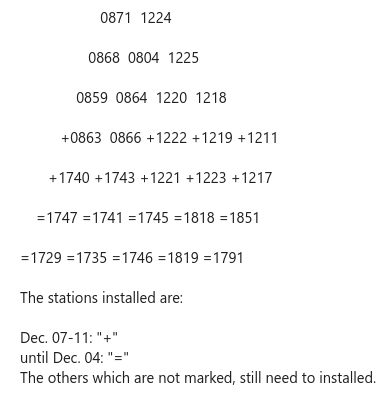
\includegraphics[width=.35\textwidth]{listStations.png}
			\end{tabular}
			&
			\begin{tabular}{l}
				\includegraphics[width=.45\textwidth]{mapStations.pdf}
			\end{tabular}
		\end{tabularx}
	\end{figure}
\end{frame}


\begin{frame}
	\frametitle{Checking Offset differences for more UUB Satations}
	{\bf Checking for LPMT1, Peak and Charge}
	\begin{figure}
		\centering
		\begin{tabularx}{\textwidth}{CC}
			\begin{tabular}{l}
				\includegraphics[width=.5\textwidth]{../plots/uubDiffOffsetPeakPMT1.pdf}
			\end{tabular}
			&
			\begin{tabular}{l}
				\includegraphics[width=.5\textwidth]{../plots/uubDiffOffsetChargePMT1.pdf}
			\end{tabular}
		\end{tabularx}
	\end{figure}
\end{frame}


\begin{frame}
	\frametitle{Checking Offset differences for more UUB Satations}
	{\bf Checking for LPMT2 and LPMT3, Peak and Charge}
	\begin{figure}
		\centering
		\begin{tabularx}{\textwidth}{CC}
			\begin{tabular}{l}
				\includegraphics[width=.38\textwidth]{../plots/uubDiffOffsetPeakPMT2.pdf}
			\end{tabular}
			&
			\begin{tabular}{l}
				\includegraphics[width=.38\textwidth]{../plots/uubDiffOffsetChargePMT2.pdf}
			\end{tabular}
			\\
			\begin{tabular}{l}
				\includegraphics[width=.38\textwidth]{../plots/uubDiffOffsetPeakPMT3.pdf}
			\end{tabular}
			&
			\begin{tabular}{l}
				\includegraphics[width=.38\textwidth]{../plots/uubDiffOffsetChargePMT3.pdf}
			\end{tabular}
		\end{tabularx}
	\end{figure}
\end{frame}


\end{document}
